\documentclass{beamer}

\usepackage{amsmath}

\usetheme{AnnArbor}
\usecolortheme{crane}
\usefonttheme[onlymath]{serif}

\title{Deep Learning - Foundations and Concepts}
\subtitle{Chapter 10. Convolutional Networks}
\author{nonlineark@github}
\date{\today}

\begin{document}

\begin{frame}
    \titlepage
\end{frame}

\begin{frame}
    \frametitle{Outline}
    \tableofcontents
\end{frame}

\section{Computer Vision}

\begin{frame}
    \frametitle{Computer vision}
    \begin{itemize}
        \item Computer vision was one of the first fields to be transformed by the deep learning revolution, predominantly thanks to the CNN architecture.
        \item Recently alternative architectures based on transformers have become competitive with convolutional networks in some applications.
        \item Some applications for machine learning in computer vision: Classification, detection, segmentation, caption generation, synthesis, inpainting, style transfer, super-resolution, depth prediction, scene reconstruction.
    \end{itemize}
\end{frame}

\begin{frame}
    \frametitle{Image data}
    \begin{itemize}
        \item The structure of an image:
        \begin{itemize}
            \item An image comprises a rectangular array of pixels.
            \item Each pixel has either a grey-scale intensity or a triplet of red, green and blue channels each with its own intensity value.
        \end{itemize}
        \item Challenges of applying neural networks to image data:
        \begin{itemize}
            \item Images generally have a high dimensionality.
            \item Image data is highly structured.
        \end{itemize}
        \item Local correlations can be used to encode strong inductive biases into a neural network, leading to models with far fewer parameters and with much better generalization accuracy.
    \end{itemize}
\end{frame}

\section{Convolutional Filters}

\begin{frame}
    \frametitle{Inductive biases}
    To exploit the two-dimensional structure of image data to create inductive biases, we can use four interrelated concepts:
    \begin{itemize}
        \item Hierarchy.
        \item Locality.
        \item Equivariance.
        \item Invariance.
    \end{itemize}
\end{frame}

\begin{frame}
    \frametitle{Feature detectors}
    Let's restrict our attention to grey-scale images first. Consider a single unit in the first layer of a neural network:
    \begin{itemize}
        \item It takes as input just the pixel values from a small rectangular region, or patch, from the image. This patch is referred to as the receptive field of that unit.
        \item The output of this unit is given by the usual functional form comprising a weighted linear combinations of the input values, which is subsequently transformed using a nonlinear activation function: $z=\mathrm{ReLU}(w^{T}x+w_{0})$.
        \item The weights themselves form a small two-dimensional grid known as a filter, sometimes also called a kernel.
        \item The unit acts as a feature detector that signals when it finds a sufficiently good match to its kernel (basic properties of inner product).
    \end{itemize}
\end{frame}

\begin{frame}
    \frametitle{Feature detectors}
    \begin{figure}
        \caption{A single unit in the first layer of a neural network}
        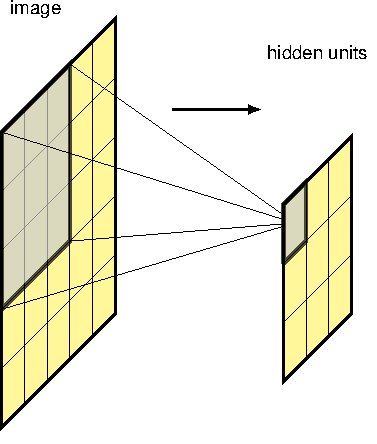
\includegraphics[height=0.7\textheight]{Figure_1_a.pdf}
    \end{figure}
\end{frame}

\begin{frame}
    \frametitle{Translation equivariance}
    \begin{itemize}
        \item To generalize what our neural network has learned in one location to all possible locations in the image, we can simply replicate the same hidden-unit weight values at multiple locations across the image.
        \item The units of the hidden layer form a feature map in which all the units share the same weights.
    \end{itemize}
    For an image $I$ with pixel intensities $I(j,k)$, and a filter $K$ with pixel values $K(l,m)$, the feature map $C$ has activation values given by:
    \begin{equation*}
        C(j,k)=\sum_{l}\sum_{m}I(j+l,k+m)K(l,m)
    \end{equation*}
    where we have omitted the nonlinear activation function for clarity. This is an example of a convolution and is sometimes expressed as $C=I*K$.
\end{frame}

\begin{frame}
    \frametitle{Translation equivariance}
    \begin{figure}
        \caption{A $3\times{}3$ image convolved with a $2\times{}2$ filter}
        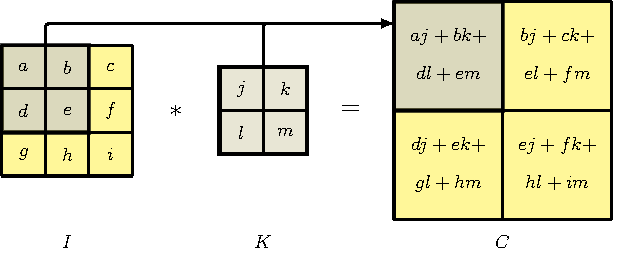
\includegraphics{Figure_3.pdf}
    \end{figure}
\end{frame}

\begin{frame}
    \frametitle{Translation equivariance}
    Comparing this convolutional structure with a standard fully connected network, we see several advantages:
    \begin{itemize}
        \item The connections are sparse, leading to far fewer weights even with large images.
        \item The weight values are shared, greatly reducing the number of independent parameters and consequently reducing the required size of the training set.
        \item The same network can be applied to images of different sizes without the need for retraining.
        \item Convolutions can be implemented very efficiently by exploiting the massive parallelism of GPUs.
    \end{itemize}
\end{frame}

\begin{frame}
    \frametitle{Padding}
    Consider an image of dimensionality $J\times{}K$ and a kernal of dimensionality $M\times{}M$:
    \begin{itemize}
        \item The feature map is of dimensionality $(J-M+1)\times(K-M+1)$, which is smaller than the original image.
        \item We can pad the original image with additional pixels around the outside. If we pad with $P$ pixels then the output map has dimensionality $(J+2P-M+1)\times(K+2P-M+1)$:
        \begin{itemize}
            \item If $P=0$, this is called a valid convolution.
            \item If $P=\frac{M-1}{2}$, this is called a same convolution.
        \end{itemize}
        \item Padding values are typically set to zero, after first subtracting the mean from each image so that zero represents the average value of the pixel intensity.
    \end{itemize}
\end{frame}

\begin{frame}
    \frametitle{Strided convolutions}
    Sometimes we wish to use feature maps that are significantly smaller than the original image to provide flexibility in the design of convolutional network architectures. One way to achieve this is to use strided convolutions in which, the filter is moved in larger steps of size $S$, called the stride. The feature map will have dimensionality:
    \begin{equation*}
        (\lfloor\frac{J+2P-M}{S}\rfloor+1)\times(\lfloor\frac{K+2P-M}{S}\rfloor+1)
    \end{equation*}
\end{frame}

\begin{frame}
    \frametitle{Multi-dimensional convolutions}
    We can easily extend convolutions to cover multiple channels by extending the dimensionality of the filter:
    \begin{itemize}
        \item An image with $J\times{}K$ pixels and $C$ channels will be described by a tensor of dimensionality $J\times{}K\times{}C$.
        \item We can introduce a filter described by a tensor of dimensionality $M\times{}M\times{}C$.
    \end{itemize}
\end{frame}

\begin{frame}
    \frametitle{Multi-dimensional convolutions}
    \begin{figure}
        \caption{A multi-dimensional filter}
        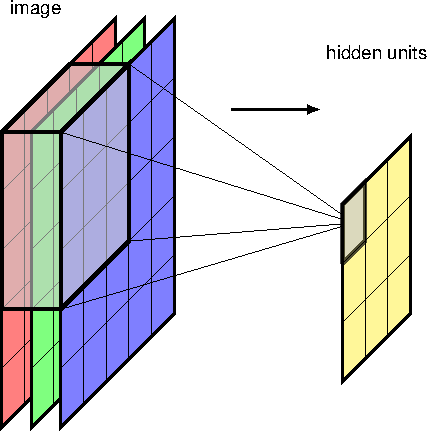
\includegraphics[height=0.7\textheight]{Figure_6_a.pdf}
    \end{figure}
\end{frame}

\begin{frame}
    \frametitle{Multi-dimensional convolutions}
    To build more flexible models, we simply include multiple filters, in which each filter has its own independent set of parameters giving rise to its own independent feature map:
    \begin{itemize}
        \item We again refer to these separate feature maps as channels.
        \item The filter tensor now has dimensionality $M\times{}M\times{}C\times{}C_{\textrm{OUT}}$ where $C$ is the number of input channels and $C_{\textrm{OUT}}$ is the number of output channels.
        \item Each output channel will have its own associated bias parameter, so the total number of parameters will be $(M^{2}C+1)C_{\textrm{OUT}}$.
    \end{itemize}
\end{frame}

\begin{frame}
    \frametitle{Pooling}
    Small changes in the relative locations do not affect the classification, and we want to be invariant to such small translations of individual features. This can be achieved using pooling:
    \begin{itemize}
        \item A pooling layer is similar to a convolutional layer:
        \begin{itemize}
            \item Each unit takes input from a receptive field in the previous feature map layer.
            \item There is a choice of filter size and of stride length.
        \end{itemize}
        \item The difference is that the output of a pooling unit is a simple, fixed function of its inputs:
        \begin{itemize}
            \item Max-pooling.
            \item Average pooling.
        \end{itemize}
    \end{itemize}
\end{frame}

\begin{frame}
    \frametitle{Pooling}
    \begin{figure}
        \caption{Illustration of max-pooling}
        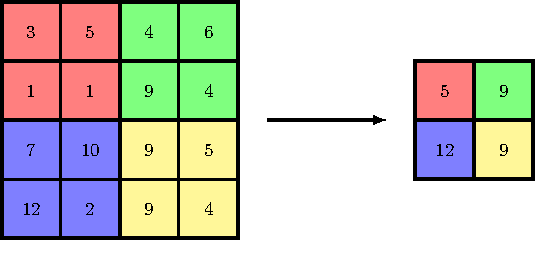
\includegraphics{Figure_8.pdf}
    \end{figure}
\end{frame}

\begin{frame}
    \frametitle{Multilayer convolutions}
    \begin{itemize}
        \item To allow the network to discover and represent hierarchical structure in the data, we extend the architecture by considering multiple layers.
        \item Each convolutional layer is described by a filter tensor of dimensionality $M\times{}M\times{}C_{\textrm{IN}}\times{}C_{\textrm{OUT}}$ in which the number of independent weight and bias parameters is $(M^{2}C_{\textrm{IN}}+1)C_{\textrm{OUT}}$.
        \item Each such convolutional layer can optionally be followed by a pooling layer.
        \item In many applications (e.g., classification tasks), the output units need to combine information from across the whole of the input image. This is typically achieved by introducing one or two standard fully connected layers as the final stages of the network.
    \end{itemize}
\end{frame}

\begin{frame}
    \frametitle{Example network architectures}
    \begin{figure}
        \caption{The architecture of a convolutional network called VGG-16}
        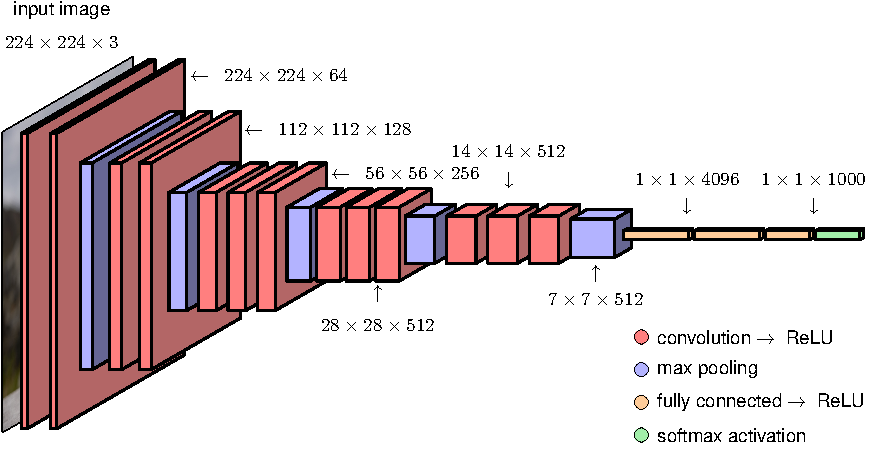
\includegraphics[width=0.8\textwidth]{Figure_10.pdf}
    \end{figure}
\end{frame}

\section{Visualizing Trained CNNs}

\begin{frame}
    \frametitle{Visual cortex}
    Historically, much of the motivation for CNNs came from pioneering research in neuroscience:
    \begin{itemize}
        \item Simple cells: Respond to visual inputs with a simple edge oriented at a particular angle and located at a particular position within the visual field.
        \item Complex cells: Respond to more complex stimuli and which seem to be derived by combining and processing the output of simple cells.
        \item Grandmother cells: Respond if, and only if, the visual input corresponds to a person's grandmother, irrespective of location, scale, lighting, or other transformations of the scene.
    \end{itemize}
\end{frame}

\begin{frame}
    \frametitle{Visual cortex}
    The response of the simple cells can be modelled using Gabor filters:
    \begin{align*}
        G(x,y)&=A\exp(-\alpha\tilde{x}^{2}-\beta\tilde{y}^{2})\sin(\omega\tilde{x}+\phi) \\
        \tilde{x}&=(x-x_{0})\cos\theta+(y-y_{0})\sin\theta \\
        \tilde{y}&=-(x-x_{0})\sin\theta+(y-y_{0})\cos\theta
    \end{align*}
    \begin{itemize}
        \item The $\sin$ term represents a sinusoidal spatial oscillation oriented in a direction defined by the polar angle $\theta$, with frequency $\omega$ and phase angle $\phi$.
        \item The exponential factor creates a decay envelope that localizes the filter in the neighborhood of position $(x_{0},y_{0})$ and with decay rates governed by $\alpha$ and $\beta$.
    \end{itemize}
\end{frame}

\begin{frame}
    \frametitle{Visual cortex}
    \begin{figure}
        \caption{Examples of Gabor filters}
        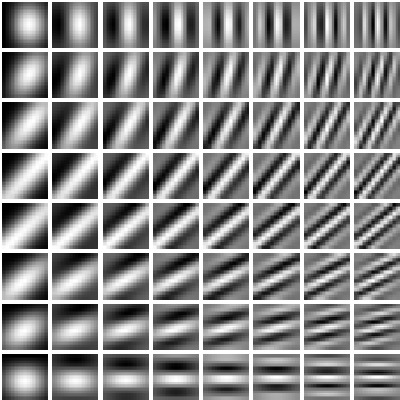
\includegraphics[height=0.7\textheight]{Figure_11.pdf}
    \end{figure}
\end{frame}

\begin{frame}
    \frametitle{Visualizing trained filters}
    For the filters in the first convolutional layer, we can visualize the network weights associated with these filters directly as small images (Cauchy-Schwarz inequality).
    \bigbreak
    We see a remarkable similarity between these filters and the Gabor filters. This is because these characteristic filters are a general property of the statistics of natural images and therefore prove useful for image understanding in both natural and artificial systems.
\end{frame}

\begin{frame}
    \frametitle{Visualizing trained filters}
    \begin{figure}
        \caption{Examples of learned filters from the first layer of AlexNet}
        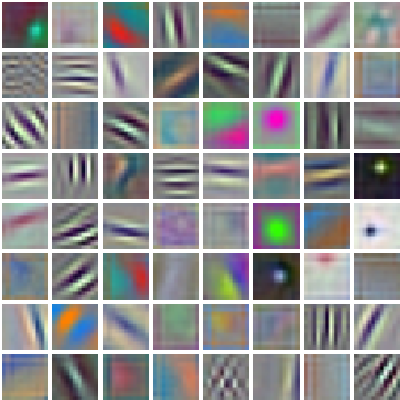
\includegraphics[height=0.7\textheight]{Figure_12.pdf}
    \end{figure}
\end{frame}

\begin{frame}
    \frametitle{Visualizing trained filters}
    One approach to visualize the filters in subsequent layers is to present a large number of image patches to the network and see which produce the highest activation value in any particular hidden unit.
    \begin{figure}
        \caption{Examples of image patches that produce the strongest activation in the hidden units in a network}
        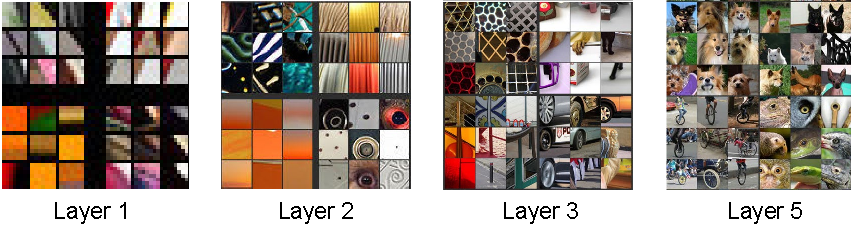
\includegraphics[width=0.8\textwidth]{Figure_13.pdf}
    \end{figure}
\end{frame}

\begin{frame}
    \frametitle{Visualizing trained filters}
    We can extend this technique to perform a numerical optimization over the input variables to maximize the activation of a particular unit. If we chose the unit to be one of the outputs then we can look for an image that is most representative of the corresponding class label.
    \begin{figure}
        \caption{Examples of synthetic images generated by maximizing the class probability}
        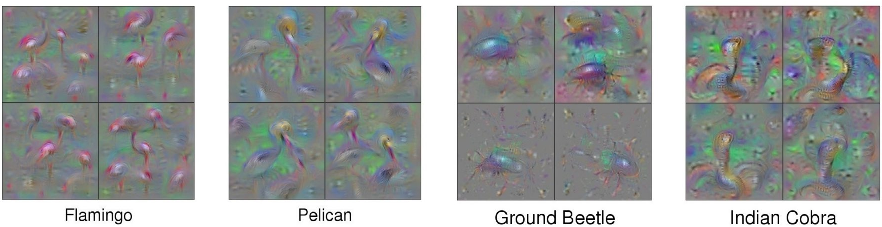
\includegraphics[width=0.8\textwidth]{Figure_14.pdf}
    \end{figure}
\end{frame}

\begin{frame}
    \frametitle{Saliency maps}
    \begin{itemize}
        \item Saliency maps aim to identify those regions of an image that are most significant in determining the class label.
        \item This is best done by investigating the final convolutional layer:
        \begin{itemize}
            \item This layer still retains spatial localization.
            \item This layer has the highest level of semantic representation.
        \end{itemize}
    \end{itemize}
\end{frame}

\begin{frame}
    \frametitle{Saliency maps}
    The Grad-CAM (gradient class activation mapping) method. For a given input image:
    \begin{itemize}
        \item First compute the derivatives of the output-unit pre-activation $a^{c}$ for a given class $c$ with respect to the pre-activations $a_{ij}^{(k)}$ of all the units in the final convolutional layer for channel $k$.
        \item For each channel in that layer, the average of those derivatives is evaluated to give: $\alpha_{k}=\frac{1}{M_{k}}\sum_{i}\sum_{j}\frac{\partial{}a^{c}}{\partial{}a_{ij}^{(k)}}$, where $M_{k}$ is the total number of units in that channel.
        \item These averages are then used to form a weighted sum of the form: $L=\sum_{k}\alpha_{k}A^{(k)}$, where $A^{(k)}$ is a matrix with elements $a_{ij}^{(k)}$.
    \end{itemize}
\end{frame}

\begin{frame}
    \frametitle{Saliency maps}
    \begin{figure}
        \caption{Saliency maps for the VGG-16 network with respect to the dog and cat categories}
        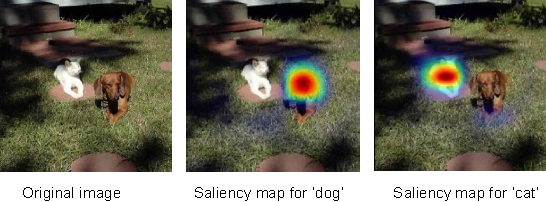
\includegraphics{Figure_15.pdf}
    \end{figure}
\end{frame}

\begin{frame}
    \frametitle{Adversarial attacks}
    \begin{itemize}
        \item Adversarial attacks involve making very small modifications to an image, at level that is imperceptible to a human, which cause the image to be misclassified by the neural network.
        \item The fast gradient sign method: Changing each pixel value in an image $x$ by a fixed amount $\epsilon$ with a sign determined by the gradient of an error function $E(x,t)$ with respect to the pixel values: $x'=x+\epsilon\mathrm{sign}(\nabla_{x}E(x,t))$, where $t$ is the true label of $x$.
    \end{itemize}
\end{frame}

\begin{frame}
    \frametitle{Synthetic images}
    DeepDream: Determine which nodes in a particular hidden layer of the network respond strongly to a particular image and then modify the image to amplify those responses:
    \begin{itemize}
        \item We apply an image to the input of the network and forward propagate through to some particular layer.
        \item We then set the backpropagation $\delta$ variables for that layer equal to the pre-activations of the nodes and run backpropagation to the input layer to get a gradient vector over the pixels of the image.
        \item Finally, we modify the image by taking a small step in the direction of the gradient vector.
    \end{itemize}
\end{frame}

\begin{frame}
    \frametitle{Synthetic images}
    \begin{figure}
        \caption{Examples of DeepDream applied to an image}
        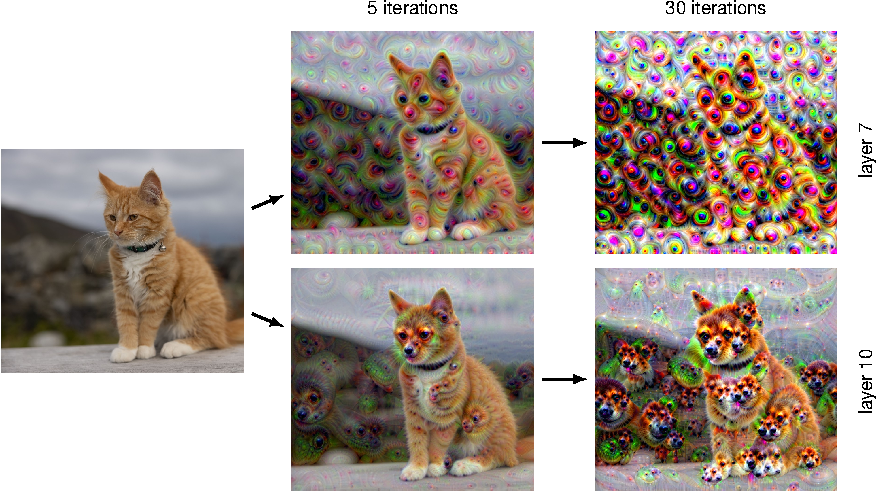
\includegraphics[height=0.6\textheight]{Figure_18.pdf}
    \end{figure}
\end{frame}

\section{Object Detection}

\begin{frame}
    \frametitle{Bounding boxes}
    \begin{itemize}
        \item When there are multiple objects in an image, we may want to detect the presence and class of each object as well as their locations.
        \item The location of an object in an image is usually defined by a bounding box: $b=(b_{x},b_{y},b_{W},b_{H})$, where $(b_{x},b_{y})$ is the coordinates of the center of the bounding box, and $b_{W}$ and $b_{H}$ its width and height.
    \end{itemize}
\end{frame}

\begin{frame}
    \frametitle{Intersection-over-union}
    \begin{itemize}
        \item We need a meaningful way to measure the performance of a trained network that can predict bounding boxes.
        \item Intersection-over-union (IoU) is the ratio of the area of the intersection of the predicted bounding box and the ground truth bounding box to that of their union:
        \begin{itemize}
            \item IoU lies in the range $[0,1]$.
            \item Predictions can be labelled as correct if the IoU exceeds a threshold, which is typically set at $0.5$.
        \end{itemize}
    \end{itemize}
\end{frame}

\begin{frame}
    \frametitle{Sliding windows}
    The sliding window way of object detection and object localization:
    \begin{itemize}
        \item Create a training set consisting of tightly cropped examples of the object to be detected, as well as examples of similarly cropped sections of images that do not contain any object (the background class).
        \item Train a classifier (e.g., a deep CNN) using the data set, whose outputs represent the probability of there being an object of each particular class in the input window.
        \item Scan an input window across the image and, for each location, taking the resulting subset of the image as input to the classifier.
        \item When an object is detected with high probability, the associated window location then defines the corresponding bounding box.
    \end{itemize}
\end{frame}

\begin{frame}
    \frametitle{Sliding windows}
    Potential drawbacks of the sliding window solution:
    \begin{itemize}
        \item It can be computationally very costly due to the large number of potential window positions in the image.
        \begin{itemize}
            \item Cost can be saved by moving the input window in strides across the image.
            \item There is a trade-off between precision of location using a small stride and reducing the computational cost by using a larger stride.
        \end{itemize}
        \item The process may have to be repeated using windows of various scales to allow for different sizes of object within the image.
    \end{itemize}
    Fortunately, it is remarkably simple to implement sliding windows efficiently in a convolutional network.
\end{frame}

\begin{frame}
    \frametitle{Sliding windows}
    \begin{figure}
        \caption{Example of a simple convolutional network}
        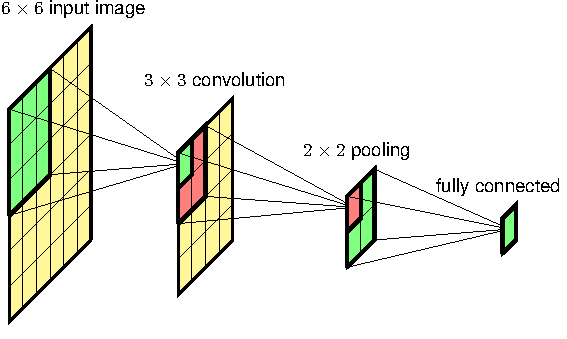
\includegraphics[height=0.7\textheight]{Figure_22.pdf}
    \end{figure}
\end{frame}

\begin{frame}
    \frametitle{Sliding windows}
    \begin{figure}
        \caption{Application of the network to a larger image}
        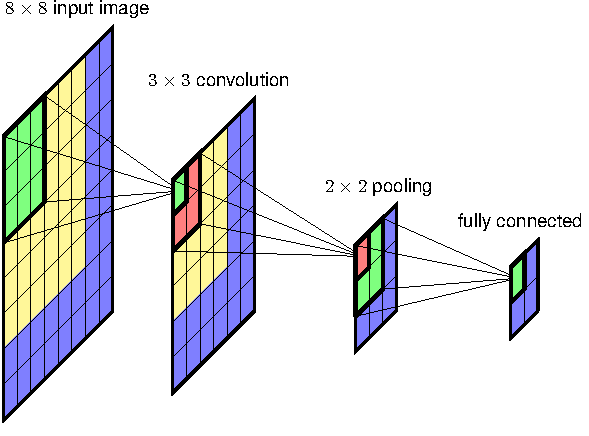
\includegraphics[height=0.7\textheight]{Figure_23.pdf}
    \end{figure}
\end{frame}

\begin{frame}
    \frametitle{Detection across scales}
    We still need to solve the problem of detecting objects at different scales and at different aspect ratios:
    \begin{itemize}
        \item {[No]} Use multiple detectors with different sizes and shapes of input window.
        \item {[Yes]} Use a fixed input window and to make multiple copies of the input image each with a different pair of horizontal and vertical scaling factors.
        \item The associated scaling factors are then used to transform the bounding box coordinates back into the original image space.
    \end{itemize}
\end{frame}

\begin{frame}
    \frametitle{Non-max suppression}
    By scanning a trained convolutional network over an image, it is possible to produce multiple detections of the same object at similar locations. This can be addressed using non-max suppression. For each object class:
    \begin{enumerate}
        \item Run the sliding window over the whole image and evaluates the probability of an object of that class being present at each location.
        \item Elimiate all the associated bounding boxes whose probability is below some threshold.
        \item The box with the highest probability is considered to be a successful detection, and the corresponding bounding box is recorded as a prediction.
        \item Any other boxes whose IoU with the successful detection box exceeds some threshold is discarded.
        \item Go to step 3 and repeat until all bounding boxes have either been discarded or declared as successful detections.
    \end{enumerate}
\end{frame}

\begin{frame}
    \frametitle{Fast region CNNs}
    Instead of applying the full power of a deep convolutional network to all areas of the image, we can apply some form of computationally cheaper technique to identify parts of the image where there is a higher probability of finding an object, and then apply the full network only to these areas:
    \begin{itemize}
        \item Fast region proposals with CNN (fast R-CNN).
        \item Use a region proposal convolutional network to identify the most promising regions: faster R-CNN.
    \end{itemize}
\end{frame}

\section{Image Segmentation}

\begin{frame}
    \frametitle{Convolutional segmentation}
    Semantic segmentation: Every pixel of an image is assigned to one of a predefined set of classes.
    \begin{itemize}
        \item Create a CNN in which each layer has the same dimensionality as the input image:
        \begin{itemize}
            \item Stride $1$ at each layer.
            \item Same padding.
            \item No pooling.
        \end{itemize}
        \item Each output unit has a softmax activation function with weights that are shared across all outputs.
        \item Such a network would still need many layers, with multiple channels in each layer, and overall this would be prohibitively costly for images of reasonable resolution.
    \end{itemize}
\end{frame}

\begin{frame}
    \frametitle{Up-sampling}
    We can create a more efficient architecture for semantic segmentation by taking a standard deep convolutional network and adding additional learnable layers that take the low-dimensional internal representation and transform it back up to the original image resolution.
    \begin{figure}
        \caption{Illustration of a CNN used for semantic image segmentation}
        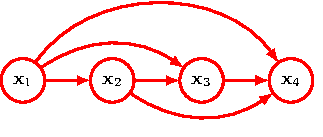
\includegraphics[width=0.8\textwidth]{Figure_27.pdf}
    \end{figure}
\end{frame}

\begin{frame}
    \frametitle{Up-sampling}
    To reverse the down-sampling effects of average pooling, we can copy over each input value into all the corresponding output units.
    \begin{figure}
        \caption{Unpooling operation for average pooling}
        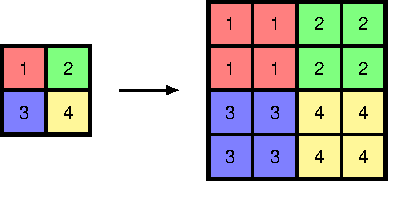
\includegraphics{Figure_28_a.pdf}
    \end{figure}
\end{frame}

\begin{frame}
    \frametitle{Up-sampling}
    To reverse the down-sampling effects of max-pooling, we can copy the input value into the first unit of the corresponding output block, and the remaining values in each block are set to zero.
    \begin{figure}
        \caption{Unpooling operation for max-pooling}
        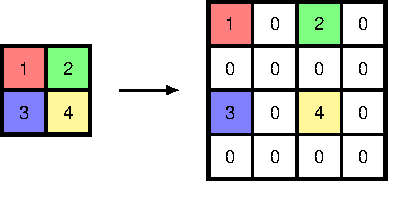
\includegraphics{Figure_28_b.pdf}
    \end{figure}
\end{frame}

\begin{frame}
    \frametitle{Up-sampling}
    Or we can:
    \begin{itemize}
        \item Choose a network architecture in which each max-pooling down-sampling layer has a corresponding up-sampling layer later in the network.
        \item During down-sampling, a record is kept of which element in each block had the maximum value.
        \item In the corresponding up-sampling layer, the non-zero element is chosen to have the same location.
    \end{itemize}
\end{frame}

\begin{frame}
    \frametitle{Up-sampling}
    \begin{figure}
        \caption{Unpooling operation for max-pooling, with spatial information kept}
        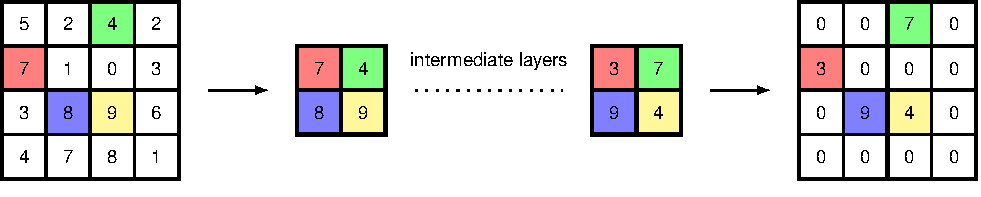
\includegraphics[width=0.8\textwidth]{Figure_29.pdf}
    \end{figure}
\end{frame}

\begin{frame}
    \frametitle{Fully convolutional networks}
    We can also use a learned up-sampling, which is the reverse of strided convolution:
    \begin{itemize}
        \item Use a filter that connects one pixel in the input array to a patch in the output array.
        \item Choose an architecture so that as we move one step across the input array, we move two or more steps across the output array.
        \item If there are output cells for which multiple filter positions overlap, we can calculate the output values by summing or by averaging the contributions from the individual filter positions.
    \end{itemize}
    If we have a network architecture with no pooling layers, so that the down-sampling and up-sampling are done purely using convolutions, then the architecture is known as a fully convolutional network.
\end{frame}

\begin{frame}
    \frametitle{Fully convolutional networks}
    \begin{figure}
        \caption{Illustration of transpose convolution}
        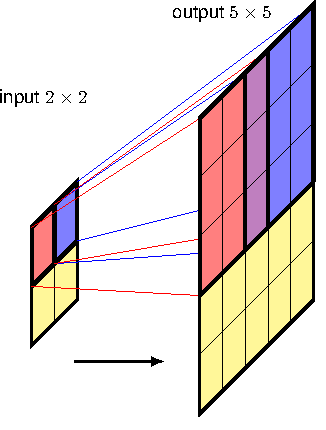
\includegraphics[height=0.7\textheight]{Figure_30.pdf}
    \end{figure}
\end{frame}

\begin{frame}
    \frametitle{The U-net architecture}
    To maintain the spatial information discarded during down-sampling, we can use the U-net architecture:
    \begin{itemize}
        \item For each down-sampling layer there is a corresponding up-sampling layer.
        \item The final set of channel activations at each down-sampling layer is concatenated with the corresponding first set of channels in the up-sampling layer.
        \item $1\times{}1$ convolutions may be used in the final layer of a U-net to reduce the number of channels down to the number of classes.
    \end{itemize}
\end{frame}

\begin{frame}
    \frametitle{The U-net architecture}
    \begin{figure}
        \caption{The U-net architecture}
        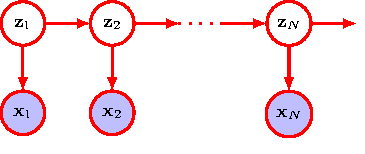
\includegraphics[width=0.8\textwidth]{Figure_31.pdf}
    \end{figure}
\end{frame}

\section{Style Transfer}

\begin{frame}
    \frametitle{Style transfer}
    Neural style transfer: Generate a synthetic image $G$ whose content is defined by an image $C$ and whose style is taken from some other image $S$. This is achieved by defining an error function $E(G)$ given by the sum of two terms:
    \begin{equation*}
        E(G)=E_{\textrm{content}}(G,C)+E_{\textrm{style}}(G,S)
    \end{equation*}
    We can then find $G$ by starting from a randomly initialized image and using gradient descent to minimize $E(G)$.
\end{frame}

\begin{frame}
    \frametitle{Style transfer}
    To define $E_{\textrm{content}}(G,C)$:
    \begin{itemize}
        \item Pick a particular convolutional layer in the network.
        \item Measure the activations of the units in that layer when image $G$ is used as input and also when image $C$ is used as input.
    \end{itemize}
    We can then encourage the corresponding pre-activations to be similar by using a sum-of-squares error function of the form:
    \begin{equation*}
        E_{\textrm{content}}(G,C)=\sum_{i,j,k}(a_{ijk}(G)-a_{ijk}(C))^{2}
    \end{equation*}
    where $a_{ijk}$ denotes the pre-activation of the unit at position $(i,j)$ in channel $k$ of that layer.
\end{frame}

\begin{frame}
    \frametitle{Style transfer}
    To define $E_{\textrm{style}}(G,S)$, the intuition is that style is determined by the co-occurrence of features from different channels within a convolutional layer. Again consider a particular convolutional layer, we can measure the extent to which a feature in channel $k$ co-occurs with the corresponding feature in channel $k'$:
    \begin{equation*}
        F_{kk'}(G)=\sum_{i=1}^{I}\sum_{j=1}^{J}a_{ijk}(G)a_{ijk'}(G)
    \end{equation*}
    where $I$ and $J$ are the dimensions of the feature maps in this particular convolutional layer. If there are $K$ channels in this layer, then $F_{kk'}$ form the elements of a $K\times{}K$ matrix, called the style matrix.
\end{frame}

\begin{frame}
    \frametitle{Style transfer}
    We can measure the extent to which the two images $G$ and $S$ have the same style by:
    \begin{equation*}
        E_{\textrm{style}}(G,S)=\frac{1}{(2IJK)^{2}}\sum_{k=1}^{K}\sum_{k'=1}^{K}(F_{kk'}(G)-F_{kk'}(S))^{2}
    \end{equation*}
    We could obtain more pleasing results by using contributions from multiple layers:
    \begin{equation*}
        E_{\textrm{style}}(G,S)=\sum_{l}\lambda_{l}E^{(l)}_{\textrm{style}}(G,S)
    \end{equation*}
    where the coefficients $\lambda_{l}$ determine the relative weighting between the different layers.
\end{frame}

\end{document}